\subsection{Problemas de falta de información}

Encontramos diferentes tipos de páginas que tenían grupos sin información e incluso páginas sin información alguna. Para guardar la información consideramos sólo los grupos que al menos tenían: nombre de profesor, número de alumnos inscritos y horario. A continuación se muestran varios ejemplos con los diferentes casos encontrados. %con falta de información.


\begin{itemize}
\item[-] En la \figurename{\ref{pagEnBlanco}} vemos un ejemplo de páginas en las cuales se tiene el nombre de la materia, pero no hay información de algún grupo: \url{http://www.fciencias.unam.mx/docencia/horarios/20081/1556/803}

\begin{figure}[H]
\centering
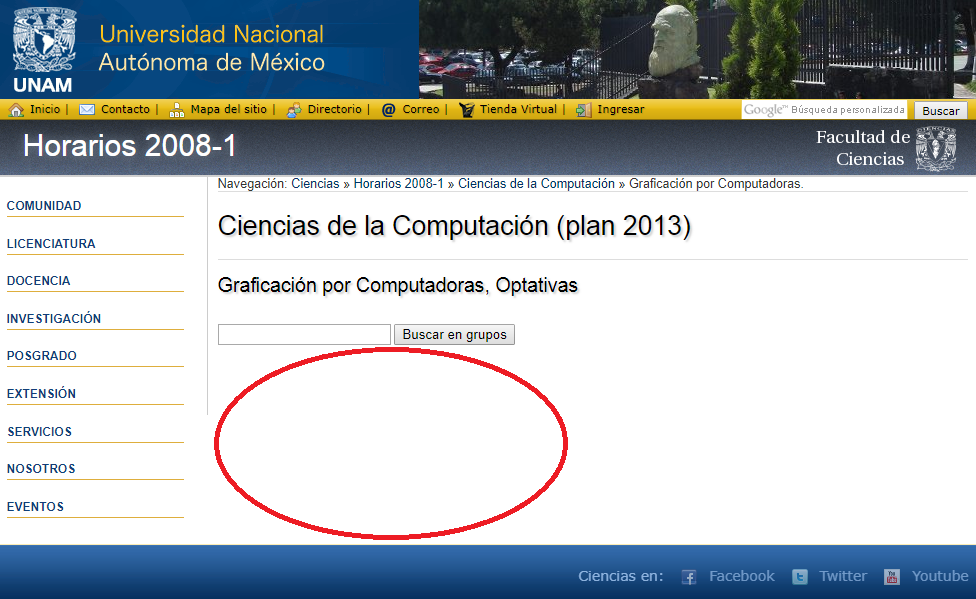
\includegraphics[scale = 0.6]{FaltaInfo_A} %width=\textwidth
\caption[\textit{Ejemplo de página web en blanco}]{\textit{Ejemplo de página web en blanco: En este tipo de páginas no encontramos información de los grupos para la materia.}}\label{pagEnBlanco}
\end{figure}

\item[-] En la \figurename{\ref{GpoSinInfo}} encontramos un ejemplo de páginas que no tienen información del salón: \url{http://www.fciencias.unam.mx/docencia/horarios/20081/119/4}

\begin{figure}[H]
\centering
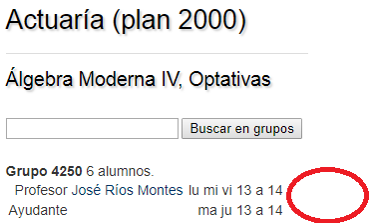
\includegraphics[scale = 0.45]{FaltaInfo_B} %width=\textwidth
\caption[\textit{Ejemplo de grupo sin información de salón}]{\textit{Ejemplo de grupo sin información de salón: En este tipo páginas no se muestra el salón en el que se imparte la clase.}}\label{GpoSinInfo}
\end{figure}

\item[-] En la \figurename{\ref{GpoSinAlumnos}} tenemos un ejemplo de páginas que tienen grupos sin información del número de alumnos inscritos en el grupo: \url{http://www.fciencias.unam.mx/docencia/horarios/20112/119/630}

\begin{figure}[H]
\centering
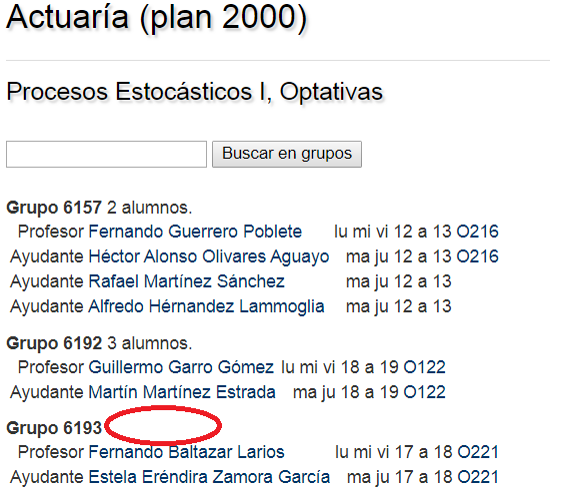
\includegraphics[scale = 0.6]{FaltaInfo_C} %width=\textwidth
\caption[\textit{Ejemplo de grupo sin información de alumnos}]{\textit{Ejemplo de grupo sin información de alumnos: En este tipo páginas encontramos grupos que no tienen el número de alumnos inscritos.}}\label{GpoSinAlumnos}
\end{figure}

\item[-] En la \figurename{\ref{SoloHorario}} vemos un ejemplo de páginas que tienen grupos sólo con el horario, sin nombre del profesor, salón, ayudante, número de alumnos, lugares disponibles: \url{http://www.fciencias.unam.mx/docencia/horarios/20091/119/841} %\url{http://www.fciencias.unam.mx/docencia/horarios/20091/119/244}

\begin{figure}[H]
\centering
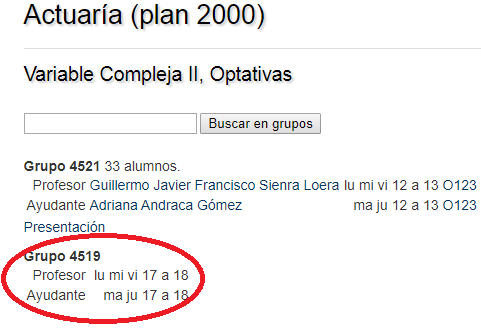
\includegraphics[scale = 0.8]{FaltaInfo_D} %width=\textwidth
\caption[\textit{Ejemplo de grupo sólo con horario}]{\textit{Ejemplo de grupo sólo con horario: En este tipo páginas existen grupos que no tienen información del profesor o salón ni del número de alumnos inscritos, sólo tienen la clave del grupo y el horario.}}\label{SoloHorario}
\end{figure}
\end{itemize}